\newvideofile{Einleitung}{Grundlagen elektrischer Netzwerke}


\s{
	\section{Einleitung}
	
	Elektrische Netzwerke sind in der heutigen Welt omnipräsent. Sie bestehen aus Zusammenschaltungen 
	von verschiedenen elektrischen Bauteilen, welche durch Verbindungsleitungen miteinander
	verknüpft sind. In der Realität kommen sie in den verschiedensten Funktionen und Größenordnungen vor. 
	So kann ein elektrisches Netzwerk sowohl eine kleine elektronische Schaltung innerhalb eines Mikrocontrolers
	mit einer Größe von einigen Mikrometern darstellen, als auch ein elektrisches Energieverteilungsnetz 
	mit Ausdehnungen von bis zu einigen 1000 Kilometern abbilden, wie sie symbolisch in den Abbildungen \ref{fig:platine} bzw. \ref{fig:stromnetz} angedeutet sind. 
	
	
	
	
	\begin{frame} 
		\begin{minipage}{0.45\textwidth}
			
			\f{width=\textwidth}{width=0.7\textwidth}{netzklein.png}{Symbolbild eines kleinen elektrischen Netzwerkes auf einer Platine  \label{fig:platine}}
			%	\fo{width=\textwidth}{width=\textwidth}{Magnetisches_Feld_Leiter}{
			%	\put(60.5, 9){\color{red}$I$}
			%	}{{\bf Magnetisches Feld um einen stromdurchflossenen Leiter.} Die Rich\-tung des Feldes kann mit der \glqq Rechten-Hand-Regel\grqq\ veranschaulicht werden.}
		\end{minipage}
		\hfill\pause
		\begin{minipage}{0.45\textwidth}
			
			\f{width=\textwidth}{width=0.7\textwidth}{netzgross.png}{Symbolbild eines großen elektrischen Netzwerkes  \label{fig:stromnetz}}
			%	\fo{width=\textwidth}{width=\textwidth}{Magnetisches_Feld_Leiterschleife}{
			%	\put(31.5, 18){\color{red}$I$}
			%	\put(65, 4){\color{red}$I$}
			%	\put(5, 37){\color{magnetfeld}N}
			%	\put(80, 79){\color{magnetfeld}S}
			%	}{{\bf Magnetisches Feld um eine stromdurchflossene, geöffnete Lei\-ter\-schleife.} Die Leiterschleife stellt die klein\-ste Einheit einer Spule dar.}
		\end{minipage}
	\end{frame}
	
	\vspace{10pt}
	
	Dieses Kapitel bietet eine Einführung zu grundlegenden Berechnungen in elektrischen Gleichstromnetzwerken.
	Ziel dieser Berechnung ist es in der Regel, die Spannungen und Ströme in allen Bauteilen des Netzwerkes
	zu berechnen. Reale Bauteile werden dazu in der Regel vereinfacht als Kombination idealer Zweipole dargestellt
	(Beispiele: Tabelle \ref{tab:schaltzeichen}). Aus der Verschaltung dieser 
	Zweipole lässt sich ein vereinfachtes Modell der realen Schaltung aufbauen, welches das grundlegende Verhalten der 
	Schaltung nachbildet.
	Dieses Modell bildet die Grundlage zur mathematischen Berechnung der Schaltung.
	
	
	Da in diesem Kapitel ausschließlich lineare Bauteile wie Widerstände oder ideale Gleichspannungsquellen verwendet werden, ist eine analytische 
	Berechnung grundsätzlich immer möglich. In fortgeschrittenen Modulen werden hingegen nichtlineare Bauelemente
	wie reale Operationsverstärker oder Dioden eingeführt. In diesem Fall ist oft eine iterative bzw. numerische Herangehensweise
	notwendig.
	
	
	
}





\begin{frame}

	\b{
		\fta{Elektrische Netzwerke}
		
		\begin{columns}
			\column[t]{0.5\textwidth}
			
			Elektrische Netzwerke bestehen aus: 
			\begin{itemize}
				\item Zwei- oder Mehrpolen: Elemente mit zwei oder mehreren el. Anschlüssen
				\item Verbunden durch ideal leitende Verbindungen
			\end{itemize}
			
			\phantom{.}\\
			
			Diese können zu Systemen unterschiedlichster Größen geschaltet werden:
			
			\begin{itemize}
				\item Energieverteilnetze \>1000 km Ausdehnung
				\item Elektronische Schaltungen im Mikrometerbereich (Mikrocontroler)
			\end{itemize}
			
			
			
			
			\column[t]{0.5\textwidth}
			
			\f{width=\textwidth}{width=0.7\textwidth}{netzgross.png}{Symbolbild eines kleinen elektrischen Netzwerkes auf einer Platine}
			\begin{center}
				Symbolbilder
			\end{center}
			
			\f{width=\textwidth}{width=0.7\textwidth}{netzklein.png}{Symbolbild eines kleinen elektrischen Netzwerkes auf einer Platine}
			
		\end{columns}
		\speech{elektrische_netzwerke}{1}{, Elektrische Netzwerke sind heute überall verbaut – in unseren Smartphones, Computern oder im riesigen Stromnetz, das ganze Städte versorgt.
			Aber was genau ist ein elektrisches Netzwerk?
			Im Grunde ist es eine Verbindung verschiedener elektrischer Bauteile über Leitungen. Diese Bauteile, wie Widerstände, Kondensatoren oder Halbleiter, übernehmen unterschiedliche Aufgaben.
			Grundsätzlich bestehen elektrische Netzwerke aus sogenannten Zwei- oder Mehrpolen – also Bauteilen mit zwei oder mehr Anschlüssen. Über diese Anschlüsse werden sie miteinander verbunden, und zwar über ideale Leitungen. Diese Leitungen haben – theoretisch – keinen eigenen Widerstand und übertragen den Strom verlustfrei.
			Elektrische Netzwerke gibt es in allen Größenordnungen:
			Winzige Schaltungen in Mikrocontrollern, kaum größer als ein Staubkorn,
			bis hin zu riesigen Energieverteilungsnetzen, die sich über tausende Kilometer erstrecken und unseren Strom liefern.}
		
		
		
	}
\end{frame}






%\begin{frame}
%	\fta{Elektrische Netzwerke}
%	\s{Während bisher die Behandlung von von wichtigen Grundbegriffen im Fokus stand, wird ab jetzt die Anwendung dieser auf Einfache Schaltungen im Vordergrund stehen.}
%	\begin{columns}
%	\column[t]{0.5\textwidth}
%	\begin{center}
%	%Motivation Zweipole: Können zu Netzwerk verschaltet werden, 
%	%wie teilen sich Strom/Spannung auf als offene Frage.
%	Ziel: Berechnung der auftretenden Größen in einer elektrischen Schaltung
%	\begin{itemize}
%		\item Vereinfachung der realen Bauteile zu idealen \textbf{Zweipolen} (Bauteile mit zwei Anschlüssen)
%		\item Darstellung der Zweipole durch Ersatzschaltbilder (siehe Tabelle)
%		\item Modellierung (Verschaltung) der idealen Zweipole zu \textbf{Netzwerken}
%		\item Modell stellt grundlegendes Verhalten der realen elektrischen Schaltung dar
%		\item vereinfachtes Modell bildet Grundlage zur mathematischen Berechnung
%	\end{itemize}
%	\end{center}
%	\column[t]{0.5\textwidth}
%	\f{width=\textwidth}{width=\textwidth}{Uebersicht_Ersatzschaltbilder.png}{Übersicht relevanter Ersatzschaltbilder}
%	Muss noch nachgebaut werden!
%	\end{columns}
%\end{frame}

%\begin{frame}
%	\fta{Elektrische Netzwerke}
%	\begin{columns}
%	\column[t]{0.5\textwidth}
%
%	Ziel: Berechnung der auftretenden Größen in einer elektrischen Schaltung
%	\begin{itemize}
%		\item Vereinfachung der realen Bauteile zu idealen Zweipolen
%		\item Darstellung der Zweipole durch Ersatzschaltbilder (siehe Tabelle)
%		\item Modellierung (Verschaltung) der idealen Zweipole
%		\item Modell stellt grundlegendes Verhalten der realen elektrischen Schaltung dar
%		\item vereinfachtes Modell bildet Grundlage zur mathematischen Berechnung
%	\end{itemize}
%	Wie teilen sich Strom und Spannung in einem Netzwerk auf?
%	\column[t]{0.5\textwidth}
%
%	Beispiele für Zweipole:
%
%
%	\begin{center}
%		\begin{tabular}{|c|c|}
%		\hline
%		Bauelement & Schaltzeichen \\
%		\hline
%		%Spannungsquelle &  \includegraphics{Uebersicht_Ersatzschaltbilder.png} \\
%		ideale Spannungsquelle & {\begin{circuitikz} \draw(0,1.5) to[european voltage source=$U_{\mathrm{0}}$] (0,0); \end{circuitikz}} \\
%		\hline
%		ideale Stromquelle & {\begin{circuitikz} \draw(0,0) to[european current source=$I_{\mathrm{0}}$] (0,1.5); \end{circuitikz}} \\
%		\hline
%		Kondensator (Kapazität) & {\begin{circuitikz} \draw(0,0) to[C] (1.5,0); \end{circuitikz}} \\
%		\hline
%		Ohmescher Widerstand & {\begin{circuitikz} \draw(0,0) to[R] (1.5,0); \end{circuitikz}} \\
%		\hline
%		Spule (Induktivität) & {\begin{circuitikz} \draw(0,0) to[L] (1.5,0); \end{circuitikz}}  \\
%		\hline
%	\end{tabular}
%	\end{center}
%	\end{columns}
%\end{frame}

\begin{frame}

	\b{
		\ftx{Elektrische Netzwerke}
		\begin{columns}
			\column[t]{0.45\textwidth}
			
			Ziel: Berechnung der elektrischen Größen in einer Schaltung
			
			\vspace{5pt}
			\begin{itemize}
				\item Vereinfachung der realen Bauteile zu idealen Zweipolen
				\item Darstellung der Zweipole durch Ersatzschaltbilder (siehe Tabelle)\\
				      $\rightarrow$ bilden Grundlage zur mathematischen Berechnung		
				\item Ersatzschaltbild modelliert grundlegendes Verhalten der realen elektrischen Schaltung
				      
			\end{itemize}
			
			\column[t]{0.55\textwidth}
			
			Beispiele für Zweipole:
			
			
			
			
			
			
			\begin{center}
				\begin{tabular}{|c|c|}
					\hline
					Zweipol & Schaltzeichen                                     \\
					\hline
					%Spannungsquelle &  \includegraphics{Uebersicht_Ersatzschaltbilder.png} \\
					%ideale Spannungsquelle
					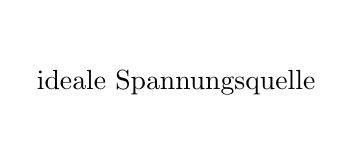
\begin{tikzpicture}[x=1mm,y=1mm]\draw[draw=none] (-10,-7) rectangle (+10,+7); \node[draw=none,align=center] {ideale Spannungsquelle};\end{tikzpicture} & {\begin{tikzpicture} \draw(0,1.5) to[european voltage source, name=V] (0,0); \draw[white] (-1.3,1.5) to[] (-1.35,1.59); \varrmore{V}{$U_0$}; \end{tikzpicture}} \\
\hline
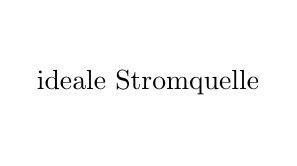
\begin{tikzpicture}[x=1mm,y=1mm]\draw[draw=none] (-10,-7) rectangle (+10,+7); \node[draw=none,align=center] {ideale Stromquelle};\end{tikzpicture} & {\begin{tikzpicture} \draw(0,0) to[european current source, name=A] (0,1.5); \iarrmore{A}{$I_0$}; \end{tikzpicture}} \\
\hline
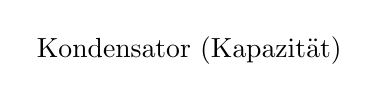
\begin{tikzpicture}[x=1mm,y=1mm]\draw[draw=none] (-10,-2) rectangle (+10,+2); \node[draw=none,align=center] {Kondensator (Kapazität)};\end{tikzpicture} & {\begin{tikzpicture} \draw(0,0) to[C] (1.5,0); \draw[white] (-0.1,-.10) to[] (0,0.5);\end{tikzpicture}} \\
\hline
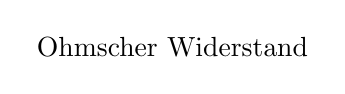
\begin{tikzpicture}[x=1mm,y=1mm]\draw[draw=none] (-10,-2) rectangle (+10,+2); \node[draw=none,align=center] {Ohmscher Widerstand};\end{tikzpicture}& {\begin{tikzpicture} \draw(0,0) to[R] (1.5,0);  \draw[white] (-0.1,-.10) to[] (0,0.35); \end{tikzpicture}} \\
\hline
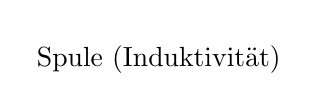
\begin{tikzpicture}[x=1mm,y=1mm]\draw[draw=none] (-10,-1) rectangle (+10,+4); \node[draw=none,align=center] {Spule (Induktivität)};\end{tikzpicture}& {\begin{tikzpicture} \draw(0,0) to[L] (1.5,0); \draw[white] (-0.1,-.10) to[] (0,0.35); \end{tikzpicture}} \\
					\hline
				\end{tabular}
			\end{center}
		\end{columns}
		
		
		\speech{folie4}{1}{Auf den folgenden Folien dieses Kapitel steigen wir in die grundlegenden Berechnungen von elektrischen Gleichstromnetzwerken ein.
			Doch was ist das eigentliche Ziel der abstrakten, mathematischen Betrachtungsweise realer Netzwerke?
			Wir wollen herausfinden, welche Spannungen und Ströme an den einzelnen Bauteilen im Netzwerk auftreten.
			Um diese Berechnungen überhaupt durchführen zu können, vereinfachen wir reale Bauteile.
			Diese werden als Kombination aus idealen Zweipolen dargestellt, Beispiele dafür findet ihr in der nebenstehenden Tabelle.
			Durch diese Vereinfachung entsteht ein Modell der Schaltung, das sich gut berechnen lässt, aber trotzdem das grundlegende Verhalten des echten Netzwerks abbildet.
			Dieses Modell bildet dann die Basis für unsere mathematischen Berechnungen.
			In diesem Kapitel verwenden wir ausschließlich lineare Bauteile, wie Widerstände und ideale Gleichspannungsquellen.
			Das hat einen großen Vorteil:
			Die Schaltungen lassen sich analytisch, also mathematisch exakt, berechnen.}
		
		
	}
\end{frame}

\newpage

\section{Zweipole und Zählpfeilsysteme}



\begin{frame}{}
	\ftx{Lernziele: Zweipole und Zählpfeilsysteme}
	
	\begin{Lernziele}{Zweipole und Zählpfeilsysteme}
		Die Studierenden können
		\begin{itemize}
			\item den Begriff des Zweipols erläutern sowie gängige Zweipole nennen und deren Schaltsymbole verwenden
			\item das Erzeuger- sowie Verbraucherzählpfeilsystem erläutern und entsprechend der Konventionen anwenden
			\item die zentralen Elemente des Grundstromkreises erläutern und die Zusammenhänge zwischen diesen erkennen
		\end{itemize}
	\end{Lernziele}
	
	\speech{folie5}{1}{Hier also nochmal zusammengefasst die Lernziele dieser Einheit:
		Nach dieser Lektion könnt ihr,
		den Begriff des Zweipols erklären, typische Zweipole benennen und ihre Schaltsymbole sicher verwenden,
		das Erzeuger- und Verbraucherzählpfeilsystem erläutern und korrekt nach den Konventionen anwenden,
		und ihr könnt die zentralen Elemente eines Grundstromkreises beschreiben und die Zusammenhänge zwischen ihnen verstehen.}
	
	
	
\end{frame}




\begin{frame}
	\ftb{Zweipole}
	
	
	\s{Als Zweipol (Abb. \ref{fig:zweipol}) wird ein Bauelement mit zwei äußeren Anschlussklemmen bezeichnet. Der innere Aufbau dieser
		Zweipole kann dabei von gänzlich unterschiedlicher Art und Komplexität sein. Beispielsweise ist ein einfacher
		elektrischer Widerstand, aber auch eine Spannungsquelle (beispielsweise eine Autobatterie) oder ein Haartrockner
		(sofern dieser nur zwei Anschlussleitungen besitzt) als Zweipol zu sehen.
		Bauteile mit mehr Anschlussleitungen werden entsprechend als Dreipol (z.B. Kühlschrank mit Schutzleiter), 
		Vierpol (z.B. Transformator) oder gar Fünfpol (elektrischer Herd mit Drehstromanschluss, Schutzleiter und Neutralleiter) bezeichnet.
		
		Unabhängig von der inneren Komplexität kann ein Zweipol im elektrischen Netzwerk vollständig durch die Beziehung von Strom
		und Spannung an seinen Anschlusspunkten, dem sogenannten \textbf{Klemmenverhalten}, charakterisiert werden. 
		Zu beachten ist dabei, dass der in Abbildung \ref{fig:zweipol} eingezeichnete Strom $I_1$ eines Zweipols stets genauso groß wie der Strom $I_2$ ist.
		
		Die praktische Realisierung der Bauteile wie reale Baumaße, Materialeigenschaften, parasitäre Effekte oder interne
		inhomogene Feldstärkeverteilungen
		werden in der Netzwerkberechnung mit Zweipolen vernachlässigt.
		
		\begin{figure}[h!]
			\begin{center}
				\begin{tikzpicture}

	\draw (0,0) rectangle (1.5,1.5);

	\draw (1.5, 1.25) to[short,i<, name=in, -o] (2.3, 1.25) node[right] {};
	\draw (1.5, 0.25) to[short,i, name=out, -o] (2.3, 0.25) node[right] {};

	\draw[white] (2.6, 1.5) to[short,v>, name=volti] (2.6, 0.0) node[right] {};

	\varrmore{volti}{$U$};
	\iarrmore{in}{$I_1$};
	\iarrmore{out}{$I_2$};

\end{tikzpicture}
			\end{center}
			\caption{Allgemeine Darstellung eines Zweipols mit den gleich großen Stromstärken $I_1$ und $I_2$ sowie der anliegender Spannung $U$}
			\label{fig:zweipol}
		\end{figure}
		
		Einige der bereits aus vorherigen Kapiteln bekannte Zweipole sind in Tabelle \ref{tab:schaltzeichen} beispielhaft aufgeführt.
		
		\begin{center}
			\begin{table}[h!]
				\centering
				\begin{tabular}{|c|c|}
					\hline
					Zweipol & Schaltzeichen                                     \\
					\hline
					%Spannungsquelle &  \includegraphics{Uebersicht_Ersatzschaltbilder.png} \\
					%ideale Spannungsquelle
					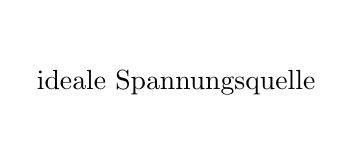
\begin{tikzpicture}[x=1mm,y=1mm]\draw[draw=none] (-10,-7) rectangle (+10,+7); \node[draw=none,align=center] {ideale Spannungsquelle};\end{tikzpicture} & {\begin{tikzpicture} \draw(0,1.5) to[european voltage source, name=V] (0,0); \draw[white] (-1.3,1.5) to[] (-1.35,1.59); \varrmore{V}{$U_0$}; \end{tikzpicture}} \\
\hline
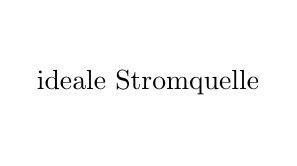
\begin{tikzpicture}[x=1mm,y=1mm]\draw[draw=none] (-10,-7) rectangle (+10,+7); \node[draw=none,align=center] {ideale Stromquelle};\end{tikzpicture} & {\begin{tikzpicture} \draw(0,0) to[european current source, name=A] (0,1.5); \iarrmore{A}{$I_0$}; \end{tikzpicture}} \\
\hline
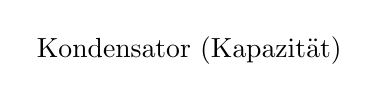
\begin{tikzpicture}[x=1mm,y=1mm]\draw[draw=none] (-10,-2) rectangle (+10,+2); \node[draw=none,align=center] {Kondensator (Kapazität)};\end{tikzpicture} & {\begin{tikzpicture} \draw(0,0) to[C] (1.5,0); \draw[white] (-0.1,-.10) to[] (0,0.5);\end{tikzpicture}} \\
\hline
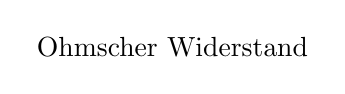
\begin{tikzpicture}[x=1mm,y=1mm]\draw[draw=none] (-10,-2) rectangle (+10,+2); \node[draw=none,align=center] {Ohmscher Widerstand};\end{tikzpicture}& {\begin{tikzpicture} \draw(0,0) to[R] (1.5,0);  \draw[white] (-0.1,-.10) to[] (0,0.35); \end{tikzpicture}} \\
\hline
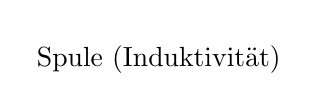
\begin{tikzpicture}[x=1mm,y=1mm]\draw[draw=none] (-10,-1) rectangle (+10,+4); \node[draw=none,align=center] {Spule (Induktivität)};\end{tikzpicture}& {\begin{tikzpicture} \draw(0,0) to[L] (1.5,0); \draw[white] (-0.1,-.10) to[] (0,0.35); \end{tikzpicture}} \\
					\hline
				\end{tabular}
				\caption{Beispiele verschiedener Zweipole sowie ihrer Schaltzeichen}
				\label{tab:schaltzeichen}
			\end{table}
		\end{center}
	}
	
	\b{
	
		\begin{columns}
			\column[t]{0.7\textwidth}
			
			Allgemein:\\
			\phantom{.}\\
			\begin{itemize}
				\item Zwei äußere Anschlüsse
				\item Klemmströme $I_1$ und $I_2$ sind gleich groß ($I_1=I_2 = I$)
				\item Klemmverhalten (Verhältnis von $I$ und $U$)
				\item Reale Baumaße, Materialeigenschaften, Feldstärkenverteilung im Bauteil werden vernachlässigt
			\end{itemize}
			
			\column[t]{0.3\textwidth}
			
			\vspace{10pt}
			
			\begin{tikzpicture}

	\draw (0,0) rectangle (1.5,1.5);

	\draw (1.5, 1.25) to[short,i<, name=in, -o] (2.3, 1.25) node[right] {};
	\draw (1.5, 0.25) to[short,i, name=out, -o] (2.3, 0.25) node[right] {};

	\draw[white] (2.6, 1.5) to[short,v>, name=volti] (2.6, 0.0) node[right] {};

	\varrmore{volti}{$U$};
	\iarrmore{in}{$I_1$};
	\iarrmore{out}{$I_2$};

\end{tikzpicture}
			
		\end{columns}
		
		\phantom{text}\\
		
		
		\textbf{Aktiver Zweiphl}: enthält Strom/Spannungsquelle(n) und ggfs. Widerstände, Kondensatoren, Spulen...\\
		
		
		\textbf{Passiver Zweipol}: Enthält keine Quellen, sondern ausschließlich Widerstände, Kondensatoren, Spulen...
		
		\begin{columns}
			\column[t]{0.6\textwidth}
			
			\column[t]{0.4\textwidth}
		\end{columns}
		
		\speech{folie6}{1}{Schauen wir uns jetzt genauer an, was ein Zweipol eigentlich ist.
			Ein Zweipol, wie rechts dargestellt, ist ein Bauelement mit genau zwei äußeren Anschlussklemmen.
			Wie komplex der innere Aufbau dieses Bauteils ist, spielt dabei erstmal keine Rolle.
			Ein einfacher Widerstand kann ein Zweipol sein, genau wie eine Spannungsquelle, etwa eine Autobatterie, oder sogar ein Haartrockner, solange er nur zwei Anschlussleitungen hat.
			Wichtig ist:
			Unabhängig von der inneren Komplexität reicht es in der Netzwerkanalyse aus, das sogenannte Klemmenverhalten zu betrachten, also die Beziehung zwischen Strom und Spannung an den Anschlussklemmen.
			Ein Punkt, den ihr euch unbedingt merken solltet:
			Der Strom, der in einen Zweipol hingeht, ist immer genauso groß wie der Strom, der auf der anderen Seite wieder herauskommt. Als Analogie könnt ihr euch hier einen Gartenschlauch vorstellen, das gesamte Wasser, das auf der einen Seite in den Schlauch geht, verlässt diesen auch wieder auf der anderen Seite.
			Zusätzlich unterscheiden wir zwischen aktiven und passiven Zweipolen:
			Ein aktiver Zweipol enthält mindestens eine Strom- oder Spannungsquelle, eventuell auch Widerstände, Kondensatoren oder Spulen.
			Ein passiver Zweipol dagegen enthält keine Quellen, sondern ausschließlich passive Bauelemente wie Widerstände, Kondensatoren oder Spulen.
			Und noch etwas:
			In unseren Berechnungen vernachlässigen wir praktische Details wie die genauen Baumaße, Materialeigenschaften oder parasitäre Effekte innerhalb des Bauteils.
			Das macht die Analyse deutlich einfacher, und trotzdem ausreichend genau für unsere Zwecke.}
		
	}
\end{frame}


\subsection{Zählpfeilsysteme}




\begin{frame}
	\ftx{Zählpfeilsysteme}
	
	\s{
	
		Die Wahl der Zählrichtungen von Strom und Spannung ist grundsätzlich beliebig. Bei der Berechnung
		elektrischer Netzwerke wird häufig versucht, die Zählrichtungen so einzuführen, dass die
		Ströme und Spannungen positiv sind. Das ist für von vornherein bekannte Größen durchaus
		sinnvoll. Für unbekannte Größen muss die Zählrichtung hingegen willkürlich festgelegt werden. Es wird
		dadurch nicht ausgedrückt, dass der Strom tatsächlich in der Pfeilrichtung fließt bzw. eine
		positive Spannung in Pfeilrichtung anliegt. Die tatsächliche Richtung wird dann durch das
		Vorzeichen der Spannung ausgedrückt.
		Für eine vorzeichengerechte Beschreibung von Strömen und Spannungen ist also eine
		Bemaßung mit Zählpfeilen zwingend notwendig.
		
		Bei Zweipolen wird zwischen den in Tabelle \ref{tab:zps} vorgestellten zwei unterschiedlichen Zählpfeilsystemen unterschieden:
		
		
		\begin{Merksatz}{Verbraucher- und Erzeugerzählpfeilsysteme}
			
			\textbf{Verbraucher-Zählpfeilsytem (VPS)}: Strom und Spannung werden am Zweipol gleichsinnig gezählt. Anzuwenden bei passiven Zweipolen (z.B. Widerständen)\\
			
			\textbf{Erzeuger-Zählpfeilsystem (EPS)}: Strom und Spannung werden am Zweipol entgegengesetzt gezählt. Anzuwendn bei aktiven Zweipolen (z.B. Spannungsquellen)
			
		\end{Merksatz}
		
		
		\begin{table}[h!]
			\centering
			\begin{tabular}{|c|c|c|c|}
				\hline
				Zählpfeilsystem & Erzeugte Leistung & Verbrauchte Leistung & Zählpfeile am Verbraucher \\ \hline
				\begin{tikzpicture}[x=1mm,y=1mm]\draw[draw=none] (-10,-10) rectangle (+10,+10); \node[draw=none,align=center] {VPS}; \end{tikzpicture} & \begin{tikzpicture}[x=1mm,y=1mm]\draw[draw=none] (-10,-10) rectangle (+10,+10); \node[draw=none,align=center] {\( P = -UI \) }; \end{tikzpicture} & \begin{tikzpicture}[x=1mm,y=1mm]\draw[draw=none] (-10,-10) rectangle (+10,+10); \node[draw=none,align=center] {\( P = UI > 0 \)}; \end{tikzpicture}  &
\begin{tikzpicture}
    \draw[white] (-0.5, 1.6) to[short,v>] (2, 1.6) node[right] {};
    \draw[white] (-0.8, 0.05) to[short,v>, name=volti] (2.3, 0.05) node[right] {};
    \draw (0,0) rectangle (1.5,1.5);

    \draw (-0.8, 0.75) to[short,i, name=in, o-] (0, 0.75) node[right] {};
    \draw (1.5, 0.75) to[short,i, name=out, -o] (2.3, 0.75) node[right] {};

    \varrmore{volti}{$U$};
    \iarrmore{in}{$I$};

\end{tikzpicture} \\ \hline
%		\begin{tikzpicture}		
%				\draw (0,0) rectangle (1.5,1.5);
%			
%				\draw (1.5, 1.25) to[short,i<, name=in, -o] (2.3, 1.25) node[right] {};
%				\draw (1.5, 0.25) to[short,i, name=out, -o] (2.3, 0.25) node[right] {};
%			
%				\draw[white] (2.6, 1.5) to[short,v>, name=volti] (2.6, 0.0) node[right] {};
%
%				\varrmore{volti}{$U$};			
%				\iarrmore{in}{$I_1$};
%\iarrmore{out}{$I_1$};

%		\end{tikzpicture} \\ \hline
\begin{tikzpicture}[x=1mm,y=1mm]\draw[draw=none] (-10,-10) rectangle (+10,+10); \node[draw=none,align=center] {EPS}; \end{tikzpicture} & \begin{tikzpicture}[x=1mm,y=1mm]\draw[draw=none] (-10,-10) rectangle (+10,+10); \node[draw=none,align=center] {\( P = UI > 0 \)}; \end{tikzpicture}  & \begin{tikzpicture}[x=1mm,y=1mm]\draw[draw=none] (-10,-10) rectangle (+10,+10); \node[draw=none,align=center] {\( P = -UI \)}; \end{tikzpicture} &



\begin{tikzpicture}
    \draw[white] (-0.5, 1.6) to[short,v>] (2, 1.6) node[right] {};
    \draw[white] (-0.8, 0.05) to[short,v>, name=volti] (2.3, 0.05) node[right] {};
    \draw (0,0) rectangle (1.5,1.5);

    \draw (-0.8, 0.75) to[short,i<, name=in, o-] (0, 0.75) node[right] {};
    \draw (1.5, 0.75) to[short,i, name=out, -o] (2.3, 0.75) node[right] {};

    \varrmore{volti}{$U$};
    \iarrmore{in}{$I$};

\end{tikzpicture} \\ \hline


%\begin{tikzpicture}
%			\draw (0,0) rectangle (1.5,1.5);
%			
%			\draw (1.5, 1.25) to[short,i, name=in, -o] (2.3, 1.25) node[right] {};
%			\draw (1.5, 0.25) to[short,i<, name=out, -o] (2.3, 0.25) node[right] {};
%		
%			\draw[white] (2.6, 1.5) to[short,v>, name=volti] (2.6, 0.0) node[right] {};
%
%				\varrmore{volti}{$U$};			
%				\iarrmore{in}{$I$};
%\iarrmore{out}{$I_1$};
%			\end{tikzpicture} \\ \hline
				
			\end{tabular}
			\caption{Vergleich zwischen Verbraucherzählpfeilsystem (VPS) und Erzeugerzählpfeilsystem (EPS).}
			\label{tab:zps}
		\end{table}
		
		
		\begin{Merksatz}{Zählpfeile}
			Zählpfeile dienen der Zählweise und sind nicht mit Vektoren zu verwechseln!
		\end{Merksatz}
		
	}
	
	
	
	\b{
		Zählpfeilrichtung theoretisch beliebig, jedoch Konventionen: 
		\begin{itemize}
			\item Verbraucher-Zählpfeilsytem (VPS): Strom und Spannung \textbf{gleichsinnig}\\
			      (passive Zweipole, z.B. Widerständen)
			\item Erzeuger-Zählpfeilsystem (EPS): Strom und Spannung \textbf{entgegengesetzt}\\
			      (aktive Zweipole, z.B. Spannungsquellen)
		\end{itemize}
		
		
		
		\begin{table}[h!]
			\centering
			\begin{tabular}{|c|c|c|c|}
				\hline
				Zählpfeilsystem & Erzeugte Leistung & Verbrauchte Leistung & Zählpfeile am Verbraucher \\ \hline
				\begin{tikzpicture}[x=1mm,y=1mm]\draw[draw=none] (-10,-10) rectangle (+10,+10); \node[draw=none,align=center] {VPS}; \end{tikzpicture} & \begin{tikzpicture}[x=1mm,y=1mm]\draw[draw=none] (-10,-10) rectangle (+10,+10); \node[draw=none,align=center] {\( P = -UI \) }; \end{tikzpicture} & \begin{tikzpicture}[x=1mm,y=1mm]\draw[draw=none] (-10,-10) rectangle (+10,+10); \node[draw=none,align=center] {\( P = UI > 0 \)}; \end{tikzpicture}  &
\begin{tikzpicture}
    \draw[white] (-0.5, 1.6) to[short,v>] (2, 1.6) node[right] {};
    \draw[white] (-0.8, 0.05) to[short,v>, name=volti] (2.3, 0.05) node[right] {};
    \draw (0,0) rectangle (1.5,1.5);

    \draw (-0.8, 0.75) to[short,i, name=in, o-] (0, 0.75) node[right] {};
    \draw (1.5, 0.75) to[short,i, name=out, -o] (2.3, 0.75) node[right] {};

    \varrmore{volti}{$U$};
    \iarrmore{in}{$I$};

\end{tikzpicture} \\ \hline
%		\begin{tikzpicture}		
%				\draw (0,0) rectangle (1.5,1.5);
%			
%				\draw (1.5, 1.25) to[short,i<, name=in, -o] (2.3, 1.25) node[right] {};
%				\draw (1.5, 0.25) to[short,i, name=out, -o] (2.3, 0.25) node[right] {};
%			
%				\draw[white] (2.6, 1.5) to[short,v>, name=volti] (2.6, 0.0) node[right] {};
%
%				\varrmore{volti}{$U$};			
%				\iarrmore{in}{$I_1$};
%\iarrmore{out}{$I_1$};

%		\end{tikzpicture} \\ \hline
\begin{tikzpicture}[x=1mm,y=1mm]\draw[draw=none] (-10,-10) rectangle (+10,+10); \node[draw=none,align=center] {EPS}; \end{tikzpicture} & \begin{tikzpicture}[x=1mm,y=1mm]\draw[draw=none] (-10,-10) rectangle (+10,+10); \node[draw=none,align=center] {\( P = UI > 0 \)}; \end{tikzpicture}  & \begin{tikzpicture}[x=1mm,y=1mm]\draw[draw=none] (-10,-10) rectangle (+10,+10); \node[draw=none,align=center] {\( P = -UI \)}; \end{tikzpicture} &



\begin{tikzpicture}
    \draw[white] (-0.5, 1.6) to[short,v>] (2, 1.6) node[right] {};
    \draw[white] (-0.8, 0.05) to[short,v>, name=volti] (2.3, 0.05) node[right] {};
    \draw (0,0) rectangle (1.5,1.5);

    \draw (-0.8, 0.75) to[short,i<, name=in, o-] (0, 0.75) node[right] {};
    \draw (1.5, 0.75) to[short,i, name=out, -o] (2.3, 0.75) node[right] {};

    \varrmore{volti}{$U$};
    \iarrmore{in}{$I$};

\end{tikzpicture} \\ \hline


%\begin{tikzpicture}
%			\draw (0,0) rectangle (1.5,1.5);
%			
%			\draw (1.5, 1.25) to[short,i, name=in, -o] (2.3, 1.25) node[right] {};
%			\draw (1.5, 0.25) to[short,i<, name=out, -o] (2.3, 0.25) node[right] {};
%		
%			\draw[white] (2.6, 1.5) to[short,v>, name=volti] (2.6, 0.0) node[right] {};
%
%				\varrmore{volti}{$U$};			
%				\iarrmore{in}{$I$};
%\iarrmore{out}{$I_1$};
%			\end{tikzpicture} \\ \hline                                          \\
			\end{tabular}
			
		\end{table}
		
		\speech{folie7}{1}{ Mit diesen Grundlagen können wir jetzt die Wahl der Zählrichtungen für Strom und Spannung betrachten. Als Zählpfeil werden die in Pfeile bezeichnet, die dem Strom beziehungsweise der Spannung zugeordnet werden. Wir brauchen Zählpfeile, damit unsere Berechnungen eindeutig sind.
			
			Grundsätzlich ist es erstmal beliebig, in welche Richtung wir Ströme und Spannungen ansetzen.
			In der Praxis wählen wir die Zählrichtungen aber oft so, dass die Ergebnisse möglichst positive Werte liefern – wenn wir die Richtung schon kennen.
			Kennen wir sie noch nicht, müssen wir die Richtung willkürlich festlegen.
			Ob unsere Annahme stimmt, zeigt sich später:,
			Ein positives Ergebnis bestätigt die Richtung,
			ein negatives Ergebnis bedeutet, dass der Strom oder die Spannung entgegen unserer Vorgabe fließt.
			Bei Zweipolen gibt es dafür zwei wichtige Zählpfeilsystem (formal in der untenstehenden Tabelle zu sehen):
			Das Verbraucher-Zählpfeilsystem, oft VPS abgekürzt: Strom und Spannung zeigen in dieselbe Richtung, dies wird typischerweise für Widerstände und andere passive Bauteile.
			Beim Erzeuger-Zählpfeilsystem oder auch EPS zeigen Strom und Spannung in dei entgegengesetzte Richtung, dieses wird oft typi bei Spannungsquellen und andere aktive Bauteile verwendet.
			Anzumerken ist jedoch folgendes:
			Zählpfeile sind keine Vektoren! Sie legen nur die Zählrichtung fest, nicht eine physikalische Richtung im Raum.
		}
		
		
	}
	
\end{frame}





%\begin{frame}
%	\fta{Elektrische Netzwerke}
%
%	\begin{columns}
%		\column[c]{0.5\textwidth}
%		Die wichtigsten Begriffe sind in der Abbildung dargestellt:
%		\begin{itemize}
%			\item idealsierte Zweipole bilden \textbf{Zweige} des Netzwerks
%			\item Verbindung der einzelnen Zweige über \textbf{Konten}
%			\item geschlossene Kette von Zweigen bildet \textbf{Masche}
%		\end{itemize}
%		Wie teilen sich Strom und Spannung in einem Netzwerk auf?
%		\column[c]{0.5\textwidth}
%		\begin{circuitikz}
%           \draw(0,0) to[R=$R_\mathrm{1}$] (0,2)
%			to[R=$R_{\mathrm{2}}$] (3,2)
%           to[V=$U_{\mathrm{0}}$,-*] (3,0)
%            to[short,-*](0,0);
%			\draw(3,0) to[R=$R_\mathrm{3}$] (3,-2)
%			to[short](0,-2)
%			to[R=$R_{\mathrm{4}}$] (0,0);
%			\draw[dashed](-0.9,-0.25) to[short] (-0.9,-2.5)
%			to[short] (3.9,-2.5)
%			to[short] (3.9,-0.25)
%			to[short] (2.5,-0.25)
%			to[short] (2.5,-1.5)
%			to[short] (0.5,-1.5)
%			to[short] (0.5,-0.25)
%			to[short] (-0.9,-0.25);
%			\draw
%			(1.5,-4.2)
%			node[label={above:$Zweig$}] {};
%			\draw
%			(4.0,0)
%			node[label={right:$Knoten$}] {};
%			\draw[->,shift={(1.5,0.6)}] (180:.8cm) arc (180:0:.8cm) node at(0,0){$Masche$};
%			\draw[->] (4,0) -- (3.2,0);
%			\draw[->] (1.5,-3.5) -- (1.5,-2.6);
%       \end{circuitikz}
%	 \end{columns}
%\end{frame}

\begin{frame}
	\ftx{Der Grundstromkreis}
	
	\subsection{Der Grundstromkreis}
	\s{
	
		Die zuvor eingeführten Zweipole (oder auch Mehrpole) lassen sich zu einem 
		elektrischen Netzwerk zusammenschließen.\\
		
		
		\begin{figure}[h!]
			\begin{center}

				\begin{tikzpicture}
    \only<1-3>{\draw(0,0) to[R=$R_1$] (0,2)
        to[R=$R_2$] (3,2)
        to[V,v,name=V,-*] (3,0)
        to[short,-*](0,0);}
    \draw(3,0) to[R=$R_3$] (3,-2)
    to[short](0,-2)
    to[R=$R_4$] (0,0);
    \only<2->{\draw[dashed, draw = teal](-0.9,-0.25) to[short] (-0.9,-2.5)
    to[short] (3.9,-2.5)
    to[short] (3.9,-0.25)
    to[short] (2.5,-0.25)
    to[short] (2.5,-1.5)
    to[short] (0.5,-1.5)
    to[short] (0.5,-0.25)
    to[short] (-0.9,-0.25);
    \draw(1.5,-4.2)node[label={above:{\textcolor{teal}{Zweig}}}] {};}
    \only<3->{\draw(3.9,0)node[label={right:{\textcolor{red}{$K_2$}}}] {};}
    \only<4>{\draw[->,draw = blue, shift={(2.9,1.05)}] (180:.8cm) arc (15:345:.7cm) node at(5,2){};}
    %\only<4->{\draw[->,draw = blue, shift={(1.5,0.6)}] (180:.8cm) arc (180:0:.8cm) node at(0,0){\textcolor{blue}{Masche}};}
    \only<3->{\draw[->, draw = red] (4,0) -- (3.2,0);}
    \only<3->{\draw[->, draw = red] (-1,0) -- (-0.2,0);}
    \only<3->{\draw(-1.2,0.3)node[label={right:{\textcolor{red}{$K_1$}}}] {};}
    \only<2->{\draw[->, draw = teal] (1.5,-3.5) -- (1.5,-2.6);}
    \draw(1.45,0.45) node[label={above:{\textcolor{blue}{$M_1$}}}] {};
    \draw[blue](0,0) to[R=\color{black}$R_1$] (0,2)
    to[R=\color{black}$R_2$] (3,2)
    to[V,v,name=V,-*] (3,0)
    to[short,-*](0,0);

    \varrmore{V}{$U_0$};
\end{tikzpicture}
				
			\end{center}
			\caption{Der elektrische Grundstromkreis mit eingezeichneten Zweigen, Knoten und Maschen}
			\label{fig:grundstromkreis}
		\end{figure}
		Dabei bilden die idealisierten Zweipole \textbf{Zweige}, die wie in Abb. \ref{fig:grundstromkreis}
		auch aus mehreren direkt hintereinandergeschalteten Zweipolen bestehen können. Durch alle Elemente eines Zweiges fließt
		der gleiche Strom. Neben dem in Abbildung \ref{fig:grundstromkreis} grün markierten Zweig bilden auch die Zweipolgruppe 
		$R_1$, $R_2$ und $U_0$ sowie der Kurzschluss in der der Zeichnung jeweils einen weiteren Zweig.\\
		
		Die Verbindungspunkte, an denen sich jeweils mindestens drei Zweige treffen, werden als \textbf{Knoten} oder Knotenpunkte
		bezeichnet. Ein fließender elektrischer Strom kann sich hier auf die verschiedenen Zweige aufteilen.
		Das elektrische Potential ist jedoch für alle verbundenen Anschlüsse identisch.
		Ein Knoten wird im Schaltplan durch einen ausgefüllten Kreis gekennzeichnet und mit $K_n$ genannt. 
		Geschlossene Pfade von mindestens zwei sich aneinanderreihenden Zweigen innerhalb 
		eines Netzwerkes werden \textbf{Maschen} genannt und mit $M_n$ abgekürzt. Im Schaltplan wird neben der Bezeichnung der Masche
		häufig auch eine Umlaufrichtung mit einem Pfeil angedeutet, der die Umlaufrichtung der Masche angibt. 
		Im hier gezeichneten Grundstromkreis lassen sich neben der eingezeichneten Masche $M_1$ bestehend aus $R_1$, $R_2$, $U_0$ und 
		dem Kurzschluss zwischen den Knoten $K_1$ und $K_2$
		zwei weitere Maschen finden: Der grün eingezeichnete Zweig zusammen mit dem Kurzschluss zwischen $K_1$ und $K_2$ bilden 
		eine Masche $M_2$. Eine weitere Masche $M_3$ außen herum führt außen um die Schaltung herum und enthält alle eingezeichneten
		Zweipole, nicht jedoch den Kurzschluss zwischen $K_1$ und $K_2$.
		
		
		
		
		
	}
	\b{
	
		\begin{columns}
			\column[c]{0.5\textwidth}
			Die wichtigsten Begriffe sind in der Abbildung dargestellt:
			\only<2->{\begin{itemize}

					\item idealsierte Zweipole bilden \textbf{Zweige} des Netzwerks
					      
					      \only<3->{\item Verbindung der einzelnen Zweige über \textbf{Knoten} $K_n$ }
					      \only<4->{\item geschlossene Kette von Zweigen bildet \textbf{Masche} $M_n$ }
				\end{itemize}
			}
			\only<7->{Wie teilen sich Strom und Spannung in einem Netzwerk auf?}
			\column[c]{0.5\textwidth}
			\begin{tikzpicture}
				\draw(0,0) to[R=$R_1$] (0,2)
				to[R=$R_2$] (3,2)
				to[V,v,name=V,-*] (3,0)
				to[short,-*](0,0);
				\draw(3,0) to[R=$R_3$] (3,-2)
				to[short](0,-2)
				to[R=$R_4$] (0,0);
				\only<2->{\draw[dashed, draw = teal](-0.9,-0.25) to[short] (-0.9,-2.5)
				to[short] (3.9,-2.5)
				to[short] (3.9,-0.25)
				to[short] (2.5,-0.25)
				to[short] (2.5,-1.5)
				to[short] (0.5,-1.5)
				to[short] (0.5,-0.25)
				to[short] (-0.9,-0.25);
				\draw
				(1.5,-4.2)
				node[label={above:{\textcolor{teal}{Zweig}}}] {};}
				\only<3->{\draw
				(4.0,0)
				node[label={right:{\textcolor{red}{Knoten}}}] {};}
				\only<4>{\draw[->,draw = blue, shift={(2.9,1.05)}] (180:.8cm) arc (15:345:.7cm) node at(5,2){};
				\draw(1.45,0.45) node[label={above:{\textcolor{blue}{$M_1$}}}] {};}
				\only<3->{\draw[->, draw = red] (4,0) -- (3.2,0);}
				\only<2->{\draw[->, draw = teal] (1.5,-3.5) -- (1.5,-2.6);}
				
				\varrmore{V}{$U_0$};
				
				\only<4>{ \draw[blue](0,0) to[R=\color{black}$R_1$] (0,2)
					to[R=\color{black}$R_2$] (3,2)
					to[V,v,name=V,-*] (3,0)
					to[short,-*](0,0);}
				
				\only<5>{\draw[->,draw = blue, shift={(2.95,-0.85)}] (180:.8cm) arc (15:345:.7cm) node at(5,2){};
				\draw(1.45,-1.45) node[label={above:{\textcolor{blue}{$M_2$}}}] {};
				\draw[blue](3,0)
				to[short,-*](0,0);
				\draw[blue](3,0) to[R=$R_3$] (3,-2)
				to[short](0,-2)
				to[R=$R_4$] (0,0);}
				
				\only<6->{\draw[->,draw = blue, shift={(2.95,0.3)}] (180:.8cm) arc (15:345:.8cm) node at(5,2){};
				\draw(1.45,-0.1) node[label={above:{\textcolor{blue}{$M_3$}}}] {};
				\draw[blue](3,0) to[R=\color{black}$R_3$] (3,-2)
				to[short](0,-2)
				to[R=\color{black}$R_4$] (0,0);
				\draw[blue](0,0) to[R=\color{black}$R_1$] (0,2)
				to[R=\color{black}$R_2$] (3,2)
				to[V,v,name=V,-*] (3,0);}
				
				
				
			\end{tikzpicture}
		\end{columns}
		\speech{folie8}{1}{ Mit den nun eingeführten Zweipolen können wir jetzt ein elektrisches Netzwerk aufbauen. Beispielhaft ist hier ein Netzwerk aus vier Widerständen und einer Spannungsquelle zu sehen.}
		\speech{folie8}{2}{ In so einem Netzwerk bilden die idealisierten Zweipole sogenannte Zweige. Ein Zweig kann auch aus mehreren hintereinandergeschalteten Zweipolen bestehen, wie hier zum Beispiel durch R3 und R4 dargestellt.
			Wichtig: Durch alle Elemente eines Zweiges fließt derselbe Strom.
		}
		\speech{folie8}{3}{ Treffen mindestens drei Zweige zusammen, entsteht ein Knoten.
			Hier kann sich der Strom aufteilen, aber das elektrische Potential ist überall gleich.
			Im Schaltplan werden Knoten mit ausgefüllten Kreisen markiert.}
		\speech{folie8}{4}{ Verbindet man mehrere Zweige zu einem geschlossenen Pfad, spricht man von einer Masche. Eine Masche wird mit einem Pfeil versehen, der die Umlaufrichtung zeigt. Hier zu sehen in blau, die Masche M1, deren Umlauf gegen den Uhrzeigersinn ist. }
		\speech{folie8}{5}{Weiter kann für den unteren geschlossenen Pfad die Masche M2 gebildet werden, bestehend aus den Widerständen R3 und R4 sowie dem Kurzschluss. Ebenfalls mit der Umlaufrichtung gegen den Uhrzeigersinn}
		\speech{folie8}{6}{Auch kann eine größere äußere Masche M3 betrachtet werden, die alle Elemente umfasst, außer den Kurzschluss. Somit ergeben sich für dieses einfache Netzwerk drei Maschen}
		\speech{folie8}{7}{ Diese Maschen können wir nun dazu verwenden, um die Frage zu beantworten, wie sich der Strom und sie Spannung in dem Netzwerk aufteilt. Dies werden wir im Folgenden mit den Kirchhoffschen Regeln machen.}
		
	}
\end{frame}
